\chapter{Multiple Integrated Applications (MIA)}
\pagestyle{fancy}

MIA is designed to be a collection of scripts, tools, programs, and commands that have been created in the past and may be useful in the future. It's original idea was a place for the original author to combine all of his previous applications and codes into one location that can be compiled cross platform. MIA is written in C++ but will contain codes that were originally designed in C\#, Java, Python, and others. MIA is created for the authors personal use but may be used by others if a need or desire arises under the terms of Antonius’ General Purpose License (AGPL). 

The MIA acronym was created by the original author for the sole purpose of this application. The design of MIA is a terminal prompt that accepts commands. There are no plans to convert MIA into a GUI application as there is currently no need; however, some elements may be programmed in that produce a GUI window for certain uses such as graphs. The MIA manual is designed to be an explanation of what MIA contains as well as a guide of how to utilize the MIA program to it's fullest. 

As MIA is continually under development, this document is also. Due to this, it may fall behind and become slightly outdated as I implement and test new features into MIA. I will attempt to keep this document up to date with all of the features MIA contains but I can only do so if time permits.

\section{Setting up the MIA Encironment for Developers}

To set up MIA for development, simply git pull the project and begin working.

\section{Setting up the MIA Environment for End Users}

\begin{enumerate}
	\item First, head to the below link. You may have to type it by hand if copy-paste does not work properly\footnote{Sometimes the ``-" is compiled through \LaTeX as different ascii characters that different pdf readers or browsers do not understand as a generic dash.}.

	\begin{lstlisting}
	https://github.com/torodean/Antonius-MIA
	\end{lstlisting}
	
	\item Select the ``Clone or Download" button then ``Download ZIP" as shown in Fig. \ref{setup01}.
	
	\begin{figure}[h]
		\centering
		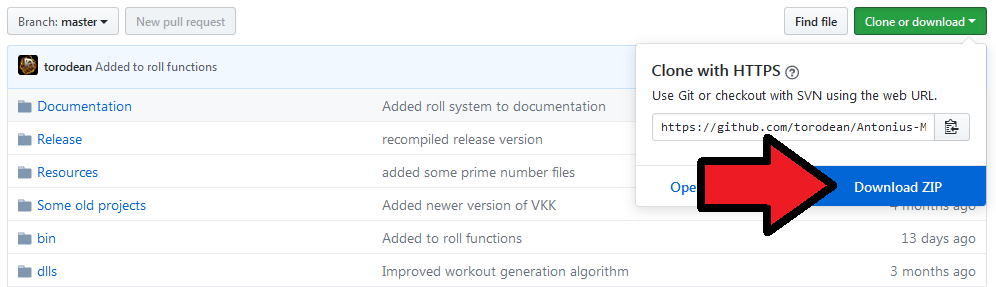
\includegraphics[width=0.9\textwidth]{Images/setup01.png}
		\caption{The release folder.} \label{setup01}
	\end{figure}
	
	\item Select ``Save File" and then press ``OK" in the window that appears. All necessary MIA files will be downloaded here. Depending on your browser (i.e Firefox, Google Chrome, Internet Explorer, etc) the downloaded files will be placed somewhere (generally the downloads folder). See Fig. \ref{setup02} for this step.
	
	\begin{figure}[h]
		\centering
		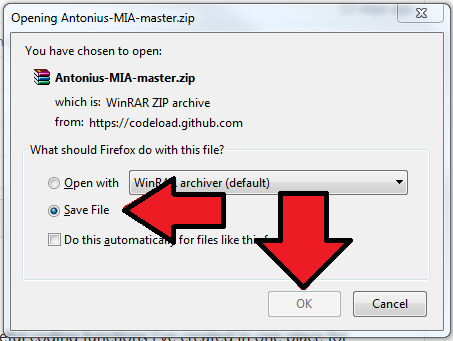
\includegraphics[width=0.4\textwidth]{Images/setup02.png}
		\caption{The release folder.} \label{setup02}
	\end{figure}
	
	\item Navigate to your downloads folder. Right click on the ``Antonius-MIA-master.zip" that should have been downloaded. If you have WinRAR installed, select ``Extract here." If you have 7-ZIP installed, select ``7-ZIP", then ``Extract here." If you have another compression software installed, figure out how to extract it. If you do not have compression software installed you can do so easily by yourself or using Ninite (https://ninite.com/). See Fig. \ref{setup03} for this step.
	
	\begin{figure}[h]
		\centering
		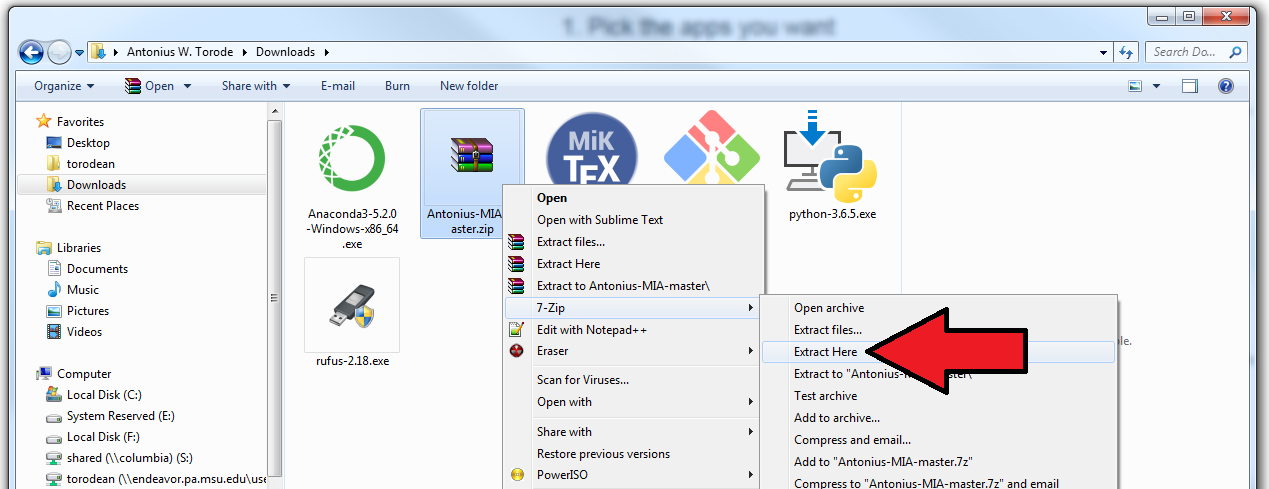
\includegraphics[width=0.9\textwidth]{Images/setup03.png}
		\caption{The release folder.} \label{setup03}
	\end{figure}

	\item If done properly, a folder will have been created in your downloads folder called ``Antonius-MIA-master." You can move this folder to wherever yo uwant the MIA program to be stored on your computer. Then, you can delete all items in the ``Antonius-MIA-master" folder EXCEPT the ``Release" folder, the ``README.md" file, and the ``Antonius’ General Purpose License (AGPL)" file. After doing so, you should be able to run and use MIA simple by opening the Release folder and clicking the ``MIA.exe" file as shown in figure \ref{setup04}.
	
	\begin{figure}[h]
		\centering
		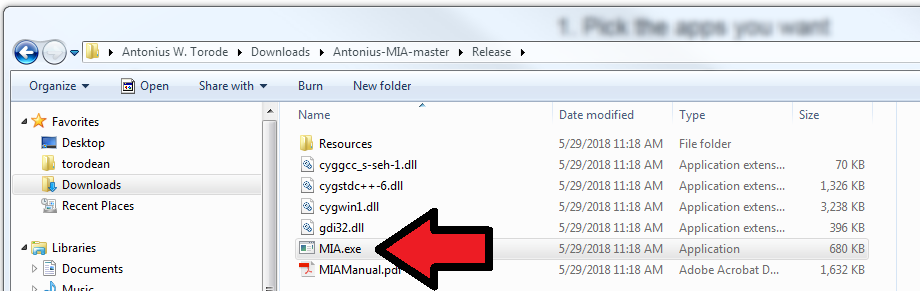
\includegraphics[width=0.9\textwidth]{Images/setup04.png}
		\caption{The release folder.} \label{setup04}
	\end{figure}

\end{enumerate}